\section{Operating principles}

Having successfully constructed the DNA nanopiston, now the operation cycle can be
discussed. For convenience, we take the rotaxane-ds configuration as the starting point
of this cycle. The power stroke of the molecular machine is initiated by bringing the
appropriate chemical fuel, ssDNA $4$ $(0.5\ \mu M)$, into solution at the trans-side. The
DNA strand is fully complementary to ssDNA $2$, thereby inducing a toehold-mediated
strand displacement. Here the flexible overhang located at the end of ssDNA $2$, referred
to as the toehold, is used to mediate the hybridisation of ssDNA $2$ and $4$ (Fig ..).

During the strand displacement reaction, two possible transient states can possibly
occur. On of the possibly scenario's describes the hybridisation happening inside of the
nanopore. This scenario is deemed to be unlikely, since this process would require three
strands of ssDNA to be simultaneously present inside the constriction of the nanopore.
Alternatively, the hybridisation can take place outside of the nanopore, in the
trans-side of the reservoir. This process implies that the neutravidin protein would
enter the lumen of the pore, which has been showed by previous studies to be possible.
This second scenario is thereby thought of as the most probable.

The resulting configuration is called the rotaxane-ss in view of the fact that it is
predominately composed of ssDNA. During this process a DNA duplex, composed of the ssDNA
2 and 4, is released into the trans-side of the reservoir.

The following step in the cycle consists of the piston's recovery stroke, induced by
bringing $0.5\ \mu M$ of ssDNA $2$ into solution at the cis-side. The strand hybridises
with the rotaxane-ss forming the rotaxane-ds structure and completing the cycle.
Each piston interaction transports one cargo strand, ssDNA $2$, from the cis- to the
trans-side of the nanopore, turning over one fuel strand in the process.


Important to note is that no external potential is specified for operating the DNA
nanopiston. In contrast to earlier DNA transporters, the piston is able to function in a
range of applied transmembrane biases. Experimentally it is verified that the
cycle operates at positive, $+20\ mV$, $+50\ mV$ and $+100\ mV$ and negative, $−20\ mV$.
The main factor determining the operational limits for a negative bias is most likely
the inability of the fuel strand to hybridise with the toehold of rotaxane-ds. The
ineptitude of the cargo to bind to the toehold is an overall limiting factor in the
operation process, resulting in faster cycles at positive then at negative applied bias
(Fig ...).

The ability of the nanopiston to transport cargo both with and against an external bias
is an important property of the molecular machine. The entropic interactions between the
DNA strands and the nanopore are expected to play an important role in this behaviour.
The piston operating at a wide range of positive biases for most likely results from the
entropic interactions between the toehold and the constricted pore entrance.  Since the
toehold is composed of flexible ssDNA is kept out the condiment of the trans-entrance to
the pore making it available for the toehold displacement reaction to happen.
After the rotaxane-ss is formed , the neutravidin protein is most likely found in the
lumen of the nanopore. The entropic interaction force resulting from the highly confined
ssDNA strand aids the rotaxane-ss to push the neutravidin bead into the cis-compartment
of the reservoir, making the hybridisation reaction possible to recover the initial
rotaxane-ds configuration.

Shows the limitation of the experimental analysis of the pore, only view into the system
is thought the measured current. To get a more in-depth understanding of the conformal
fluctuations of the pore  computation analysis was performed in the form of molecular
dynamics simulations.


% Figure 2.2a shows the measured current over through the nanopore during the operation
% cycle. The ionic current of rotaxane-ss is lower than the blocked current ofrotaxane-ds
% most likely reflecting the coiled structure of ssDNA inside the nanopore. Shows the
% limitation of the experimental analysis of the pore, only view into the system is
% throught the measured current. To get a more in-depth understanding of the conformal
% fluctuations of the pore computation analysis was performed in the form of molecular
% dynamics simulations.


%  ⡏⢱ ⠄ ⣰⡀   ⣀⡀ ⢀⡀ ⢀⡀   ⢀⡀ ⡀⣀ ⢀⡀ ⢀⡀ ⣀⡀ ⢀⣀   ⣇⡀ ⠄ ⠠   ⢀⣀ ⢀⣀ ⣇⡀ ⡀⣀ ⠄ ⠠ ⡀⢀ ⢀⡀ ⣀⡀
%  ⠧⠜ ⠇ ⠘⠤   ⠇⠸ ⠣⠜ ⣑⡺   ⠣⠭ ⠏  ⣑⡺ ⠣⠭ ⠇⠸ ⠭⠕   ⠧⠜ ⠇ ⡸   ⠭⠕ ⠣⠤ ⠇⠸ ⠏  ⠇ ⡸ ⠱⠃ ⠣⠭ ⠇⠸
% -----------------------------------------------------------------------------------------

% misschien bij de biological nanopores.
% Electrophoretic, electro-osmotic and entropic forces are, in principle, acting on the
% rotaxanes. The electrophoretic force sets the negatively charged DNA in motion, under the
% action of the applied bias (from cis to trans for
% ∆?? > 0 ). Electroosmosis generates an opposing force, arising from the motion of cations
% accumulated on the walls of the negatively charged ClyA pore and the DNA thread. Finally,
% the entropic force is solely geometry specific, and pushes the rotaxane towards
% conformations with high configurational entropy. Entropic forces are expected to play an
% important role in the rotaxanes studied here, which are composed of stiff dsDNA and
% flexible ssDNA parts.



\begin{figure}[ht]
  \begin{centering}
  \adjustbox{minipage=1.3em,valign=t}{\subcaption{}\label{sfig:testa}}%
  \begin{subfigure}[t]{\dimexpr.95\linewidth-1.3em\relax}
  \centering
  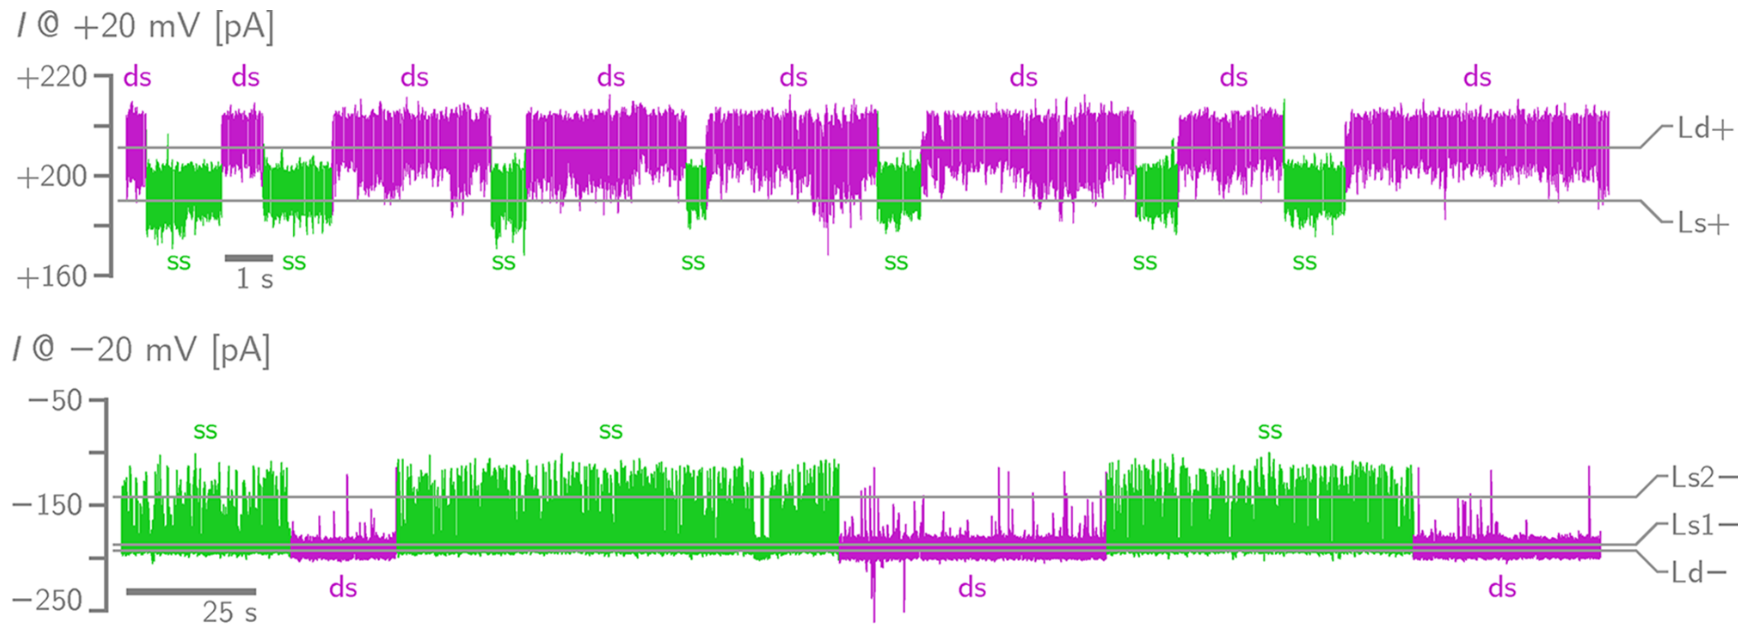
\includegraphics[width=\linewidth,valign=t]{Figures/FluctuationRotaxane.png}
  \end{subfigure}%
  \vspace{0.5cm}
  \adjustbox{minipage=1.3em,valign=t}{\subcaption{}\label{sfig:testb}}%
  \begin{subfigure}[t]{\dimexpr.5\linewidth-1.3em\relax}
  \centering
  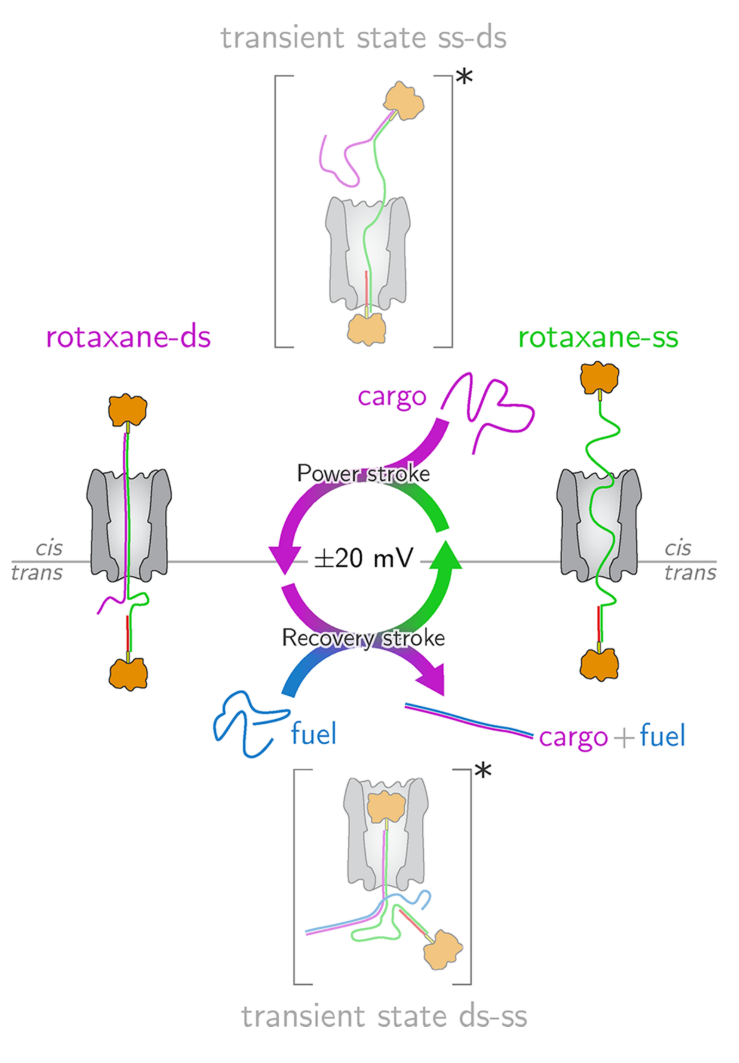
\includegraphics[width=\linewidth,valign=t]{Figures/RotaxaneCycle.png}
  \end{subfigure}
  \caption{This is a figure}
  \label{fig:test}
  \end{centering}
\end{figure}
